\newthought{\textbf{Muhammad Munawir - 2020903430026 - TRKJ 3B}}

\newday{\textbf{1 - 2 Desember 2022} - Instalasi dan Konfigurasi Apache Hadoop}
\begin{enumerate}
\item Kendala dan Solusi
\begin{itemize}
\item Kendala: \\
Saat melakukan download hadoop, terkendala dengan space disk virtual box yang tidak cukup. Saat melakukan konfigurasi apache hadoop, tidak dapat menjalankan format-hdfs. 

\item Solusi: \\
Karena virtual box tidak bisa menambahkan kapasitas space seperti di VMware. Maka melakukan instalasi ulang ubuntu. Kemudian download hadoop berhasil.
Karena tidak dapat menjalankan format-hdfs, jadi mencoba konfigurasi ulang. dan hasilnya berhasil. dan saat menjalankan test jps, hasilnya ada 5 keluaran.
\end{itemize}

\item Kesimpulan \\
Praktikum penginstalan hadoop dan konfigurasi hadoop berhasil dijalankan sesuai perintah-perintah yang ada.

\begin{figure}[!ht]
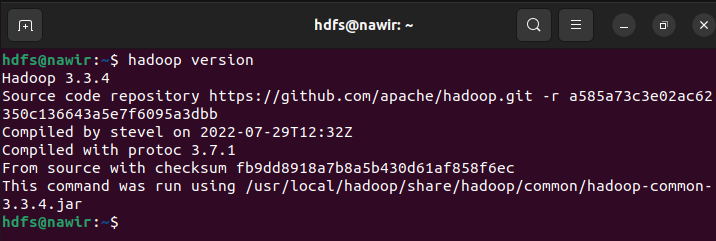
\includegraphics[width=\textwidth]{MuhammadMunawir/InstalasiHadoop}
\caption{hasil dari cek versi hadoop}
\end{figure}

\begin{figure}[!ht]
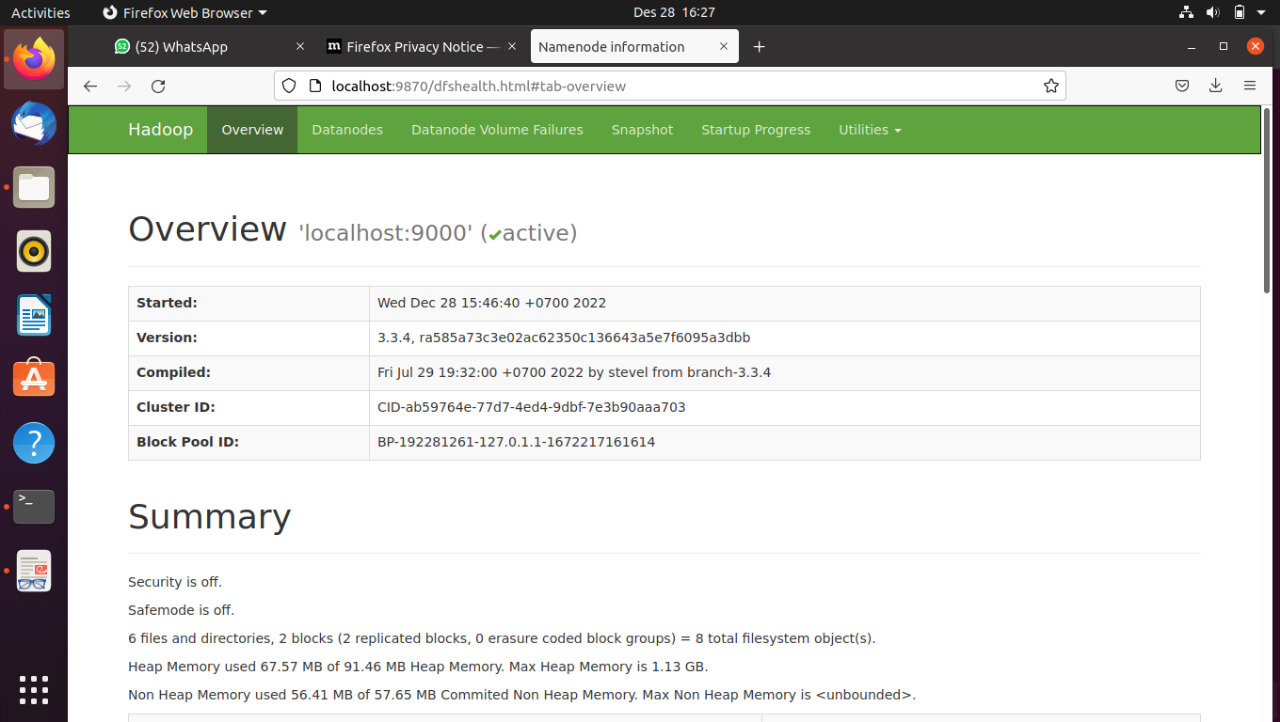
\includegraphics[width=\textwidth]{MuhammadMunawir/localhost9870}
\caption{hasil dari localhost:9870}
\end{figure}

\begin{figure}[!ht]
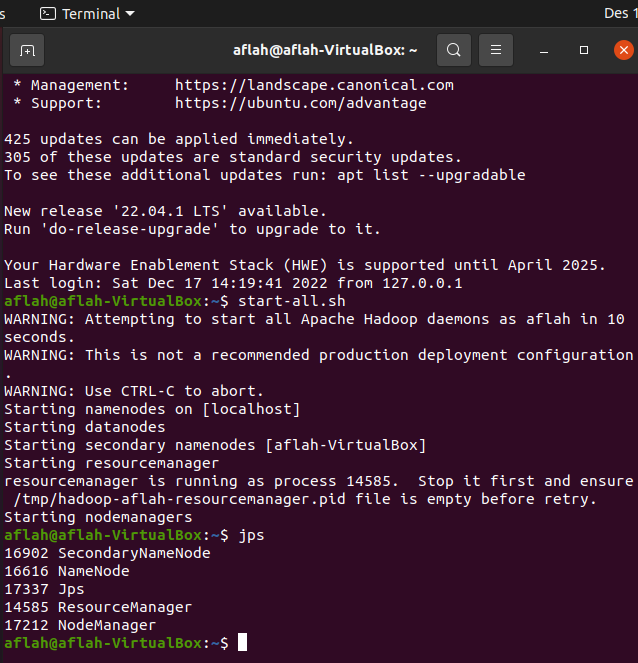
\includegraphics[width=\textwidth]{MuhammadMunawir/jps}
\caption{hasil dari menjalankan jps}
\end{figure}

\begin{figure}[!ht]
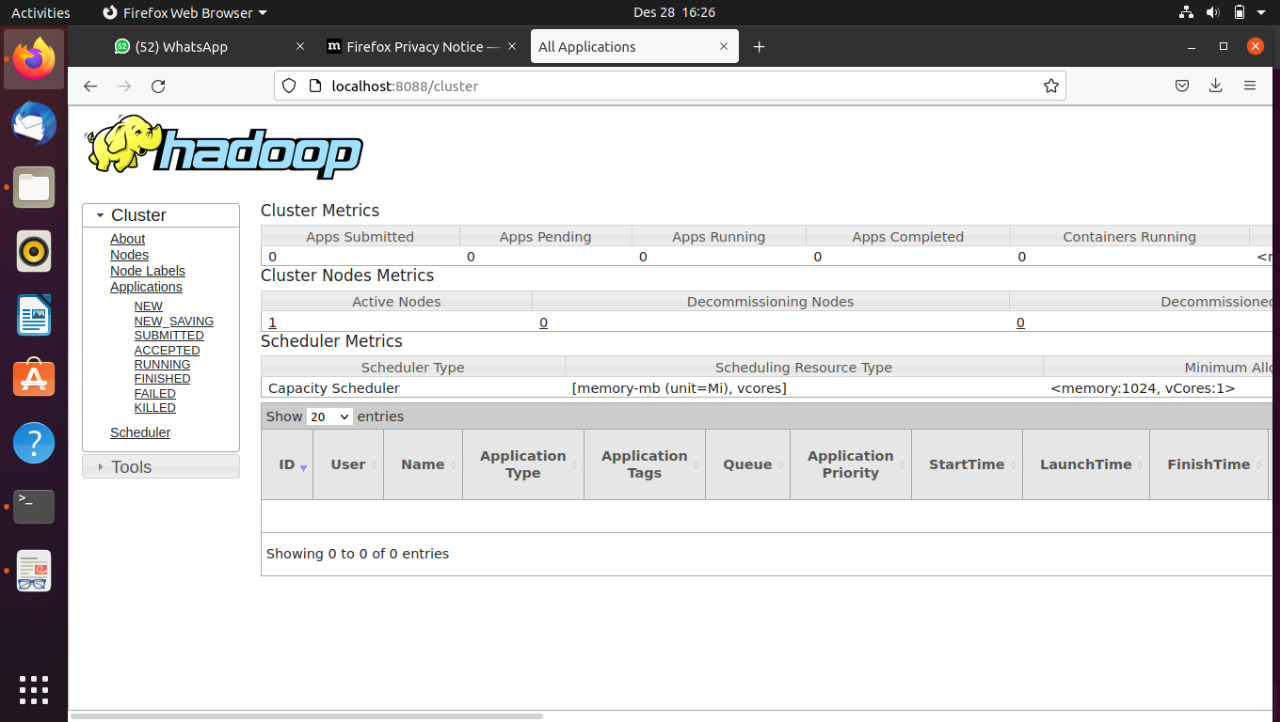
\includegraphics[width=\textwidth]{MuhammadMunawir/localhost8088}
\caption{hasil dari localhost:8088}
\end{figure}

\end{enumerate}

\newday{\textbf{15 Desember 2022} - WordCount bawaan Hadoop}
\begin{enumerate}
\item Kendala dan Solusi \\
Saat mencoba melakukan perintah/program WordCount bawaan hadoop, langakah ke 5. dimana muncul pemberitahuan untuk \textbf{"apt install emboss"}. setelah mencoba menjalankan perintah "sudo apt install emboss" dan mencoba konfigurasi ulang WordCount. Program WordCount dapat berjalan.

\begin{figure}[!ht]
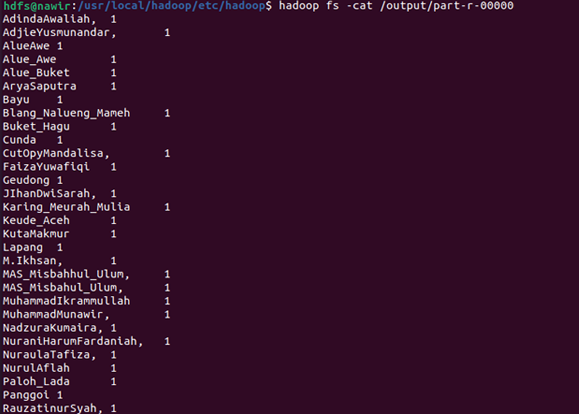
\includegraphics[width=\textwidth]{MuhammadMunawir/wordcountHadoop}
\caption{hasil dari WordCount bawaan hadoop}
\end{figure}

\item Kesimpulan \\
Program WordCount bawaan hadoop atau hadoop itu sendiri sedikit sensitif, soalnya sedikit kesalahan Program atau aplikasi pendukung yang kurang. Maka WordCount hadoop tidak dapat dijalankan.
\end{enumerate}

\newday{\textbf{16 Desember 2022} - WordCount dengan Java}
\begin{enumerate}
\item Kendala dan Solusi \\
% jelaskan kendala dan penyebab yang dialami saat mengikuti praktikum serta solusi atau langkah-langkah yang telah dilakukan
Kendala dan Solusi Pada pertemuan hari ini, kegiatan yang dilakukan adalah mencoba program wordcount dengan java. Selama praktikum mengalami kendala pada poin ke-6 berdasarkan urutan di modul. Program tidak mau dicompile karena kesalahan penulisan perintah.

\begin{figure}[!ht]
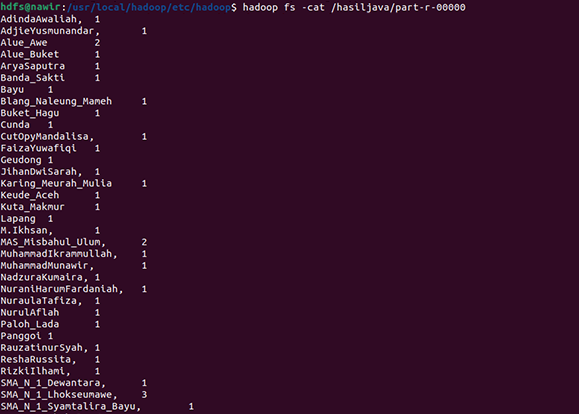
\includegraphics[width=\textwidth]{MuhammadMunawir/wordcountJava}
\caption{hasil dari WordCount dengan Program Java}
\end{figure}

\item Kesimpulan \\
% berikan kesimpulan dari praktikum yang telah dikerjkan
Dapat memberikan pemahaman dasar mengenai proses program WordCount java, dan meng-compile Program hingga menjalankan program.
\end{enumerate}

\newday{\textbf{22 Desember 2022} - Instalasi Apache Spark (PySpark)}
\begin{enumerate}
\item Kendala dan Solusi \\
Tidak ada kendala saat proses intalasi

\item Kesimpulan \\
Proses penginstalan Apache Spark berhasil dilakukan tanpa
adanya kendala satupun

\begin{figure}[!ht]
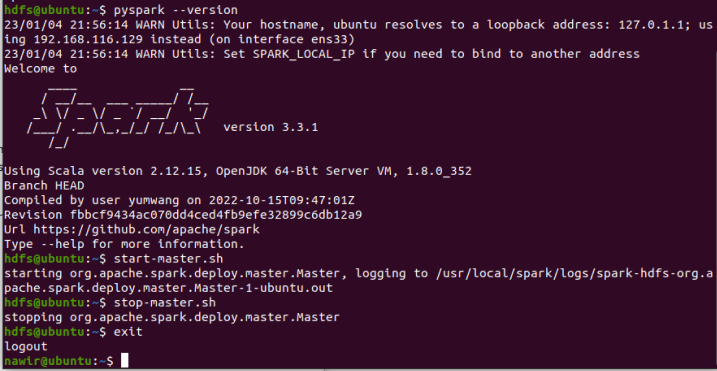
\includegraphics[width=\textwidth]{MuhammadMunawir/pysparkVersion}
\caption{hasil dari instalasi PySpark}
\end{figure}

\end{enumerate}